\providecommand{\Fun}{\operatorname{Fun}}
\providecommand{\Cat}{\mathcal{C}at}
\providecommand{\QCat}{\mathcal{Q}\mathcal{C}at}
\providecommand{\sSet}{s\mathcal{S}et}
\providecommand{\qcOne}{\mathbf{1}}   %
\providecommand{\qcTwo}{\mathbf{2}}   %
\providecommand{\qcThree}{\mathbf{3}} %

\section{\trAdjunction{}与\trEquivalence}\label{sec:adjunctions-equivalences}

在 1.4 节中，我们遇到过 2-\trCategory{}中一对对象之间\emph{\trEquivalence}的定义。
当周围的 2-\trCategory{}是某个\trInfinityCosmos{}的\trHomotopyTwoCategory{}时，
定理 1.4.7 观察到：2-范畴式的\trEquivalence{}概念恰好重新捕捉了整个%
\trInfinityCosmos{}中\trInfinityCategory{}之间的\trEquivalence{}概念。
在我们考察过的每个\trInfinityCosmos{}例子中，\trInfinityCosmos{}里可表示地定义的%
\trEquivalence{}都与该特定模型中呈现的\trInfinityCategory{}之间\trEquivalence{}的
标准概念相重合。\footnote{例如，如题外话 1.2.13 中所述，例 1.2.24 的%
\trInfinityCosmos{}中的\trEquivalence{}重新捕捉了通常\trModelStructure{}中%
\trFibrant--\trCofibrant{}对象之间的\trWeakEquivalence{}。%
}因此，2-范畴式的\trEquivalence{}概念就是\trInfinityCategory{}之间\trEquivalence{}的
「正确」概念。

类似地，2-\trCategory{}中一对对象之间的\emph{\trAdjunction{}}有一个标准定义；把它
诠释到某个\trInfinityCosmos{}中\trInfinityCategory{}、\trFunctor{}与%
\trNaturalTransformation{}的\trHomotopyTwoCategory{}上，将会给出\trInfinityCategory{}%
之间\trAdjunction{}的正确概念。

\begin{definition}[\trAdjunction]\label{def:adjunction}
\trInfinityCategory{}之间的一个\textbf{\trAdjunction}（adjunction）由下列数据构成：

\begin{itemize}
\item 一对\trInfinityCategory $A$ 与 $B$；
\item 一对\trInfinityFunctor{} $u\colon A\to B$ 与 $f\colon B\to A$；以及
\item 一对\trInfinityNaturalTransformation
$\eta\colon\mathrm{id}_B\Rightarrow uf$ 与 $\epsilon\colon fu\Rightarrow\mathrm{id}_A$，
分别称为\textbf{\trUnit}（unit）与\textbf{\trCounit}（counit），
\end{itemize}
使得\trTriangleEqualities{}成立：\footnote{左侧这对粘贴图等式断言了%
\trHomCategory{} $\mathrm{h}\Fun(\mathcal{A},\mathcal{B})$ 中的复合关系
$u\epsilon\cdot\eta u=\mathrm{id}_u$，而右侧等式断言
$\epsilon f\cdot f\eta=\mathrm{id}_f$ 于 $\mathrm{h}\Fun(\mathcal{B},\mathcal{A})$
中。粘贴图的演算在 B.1 节中综述。%
}%
\begin{center}
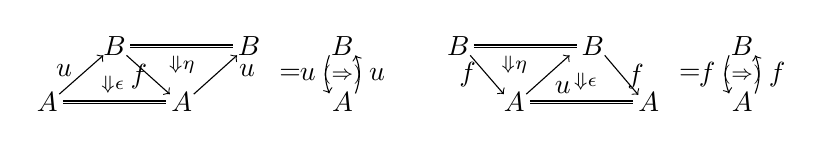
\begin{tikzpicture}[x=1.35em,y=1.35em]
  \node (A1) at (0,0) {$A$};
  \node (A2) at (3.6,0) {$A$};
  \node (B1) at (1.8,1.5) {$B$};
  \node (B2) at (5.4,1.5) {$B$};
  \draw[double] (0.42,0) -- (3.18,0);
  \draw[double] (2.22,1.5) -- (4.98,1.5);
  \draw[->] (0.32,0.22) -- (1.5,1.26);
  \node at (0.45,0.85) {$u$};
  \draw[->] (2.12,1.26) -- (3.28,0.22);
  \node at (2.45,0.68) {$f$};
  \draw[->] (3.92,0.22) -- (5.08,1.26);
  \node at (5.35,0.85) {$u$};
  \node at (1.75,0.48) {$\scriptstyle\Downarrow\epsilon$};
  \node at (3.6,1.0) {$\scriptstyle\Downarrow\eta$};
  \node at (6.5,0.75) {$=$};
  \node (Bs) at (7.9,1.5) {$B$};
  \node (As) at (7.9,0) {$A$};
  \draw[->] (7.55,1.26) to[bend right=20] node[left]{$u$} (7.55,0.24);
  \draw[->] (8.25,0.24) to[bend right=20] node[right]{$u$} (8.25,1.26);
  \node at (7.9,0.75) {$\scriptstyle(\Rightarrow)$};
  \node (B3) at (11.0,1.5) {$B$};
  \node (B4) at (14.6,1.5) {$B$};
  \node (A3) at (12.5,0) {$A$};
  \node (A4) at (16.1,0) {$A$};
  \draw[double] (11.42,1.5) -- (14.18,1.5);
  \draw[double] (12.92,0) -- (15.68,0);
  \draw[->] (11.32,1.26) -- (12.22,0.22);
  \node at (11.25,0.75) {$f$};
  \draw[->] (12.82,0.22) -- (13.98,1.26);
  \node at (13.8,0.4) {$u$};
  \draw[->] (14.92,1.26) -- (15.82,0.2);
  \node at (15.75,0.68) {$f$};
  \node at (12.5,1.0) {$\scriptstyle\Downarrow\eta$};
  \node at (14.4,0.55) {$\scriptstyle\Downarrow\epsilon$};
  \node at (17.2,0.75) {$=$};
  \node (Bt) at (18.6,1.5) {$B$};
  \node (At) at (18.6,0) {$A$};
  \draw[->] (18.25,1.26) to[bend right=20] node[left]{$f$} (18.25,0.24);
  \draw[->] (18.95,0.24) to[bend right=20] node[right]{$f$} (18.95,1.26);
  \node at (18.6,0.75) {$\scriptstyle(\Rightarrow)$};
\end{tikzpicture}
\end{center}
\trFunctor $f$ 称为\textbf{\trLeftAdjoint}（left adjoint），$u$ 称为\textbf{\trRightAdjoint}
（right adjoint）；这一关系在行文中记作 $f\dashv u$，在展示图中则画成
诸如\footnote{有些作者调整伴随图的朝向，使\trLeftAdjoint{}总取某个特定的方向；我们则改用
十字转门符号「$\dashv$」来标明哪个伴随是\trLeftAdjoint{}。}%
的图：
\begin{center}
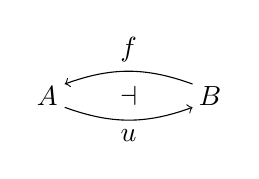
\begin{tikzpicture}[x=1.4em,y=1.4em]
  \node (A) at (0,0) {$A$};
  \node (B) at (4.2,0) {$B$};
  \draw[->] (3.75,0.3) to[bend right=20] node[above]{$f$} (0.45,0.3);
  \node at (2.1,0) {$\dashv$};
  \draw[->] (0.45,-0.3) to[bend right=20] node[below]{$u$} (3.75,-0.3);
\end{tikzpicture}
\end{center}
对\trInfinityCategory{}之间的\trFunctor{}与\trNaturalTransformation{}，
我们通常省略前缀「∞」。
\end{definition}

\begin{digression}[为伴随的 2-范畴式定义辩护]\label{dig:justifying-2categorical-adjunction}
对于觉得\cref{def:adjunction}难以置信——也许简单得让人不敢信任——的读者，
我们愿费少许笔墨作些辩护。率先提议用标准的 2-范畴式定义来定义\trInfinityCategory{}%
之间的\trAdjunction{}的是 Joyal：他在文献 \cite{bib63} 的前言中把\trQuasiCategory{}%
之间的\trAdjunction{}定义为\trHomotopyTwoCategory{} $\mathrm{h}\QCat$ 中的%
\trAdjunction{}。然而这一定义并未被广泛采纳，多数实践者改用 Lurie 的%
\trQuasiCategory{}之间\trAdjunction{}的定义 \cite[\S 5.2]{bib78}，后者取相当
不同的形式。在 F.5 节中，我们将证明：在\trQuasiCategory{}的\trInfinityCosmos{}中，
Joyal 的 2-范畴式\trAdjunction{}定义恰好复原 Lurie 的定义。如第 III 部分所解释的，
例 1.2.24 所描述的 $(\infty,1)$-\trCategory{}的各个模型都「具有同一种范畴论」，
故\cref{def:adjunction}与 $(\infty,1)$-\trCategory{}之间\trAdjunction{}的
共同体共识概念相一致。

在对象为 $(\infty,n)$- 或 $(\infty,\infty)$-\trCategory{}的那些\trInfinityCosmos{}中，
在\trHomotopyTwoCategory{}中定义的\trAdjunction{}是「伪式」（pseudo-style）%
\trAdjunction{}。它们虽不是所能考虑的最一般的\trAdjunction{}——比如，\trTriangleEqualities
关系可以只在相干的不可逆 3-\trCell{}层面成立——但它们是\trAdjunction{}的一个重要
类。\cref{def:adjunction}在一切\trInfinityCosmos{}中都相关的理由之一，在于它与%
\trEquivalence{}的关系——定理 1.4.7 确立这种\trEquivalence{}在实质上是「正确」的——
以及它与即将引入的\trLimit{}与\trColimit{}概念的关系。

最后，一种合理的异议是：\cref{def:adjunction}显得太「低维」，其数据完全落在%
\trHomotopyTwoCategory{}之中而无视\trInfinityCosmos{}中更高维的态射。事实上，
\trInfinityCategory{}之间的任何\trAdjunction{}都可扩充为一份涉及所有维数的%
\emph{\trHomotopyCoherentAdjunction}（homotopy coherent adjunction）数据，而且这种扩充在
同伦意义上唯一 \cite{bib109}。
\end{digression}

\cref{def:adjunction}所给出的\trAdjunction{}定义带有「等式式」的特征：它以
2-\trCategory{}的对象、1-\trCell{}与 2-\trCell{}及其复合来陈述。立即可得：

\begin{lemma}\label{lem:adjunction-preserved-by-2-functor}
2-\trCategory{}中的\trAdjunction{}被任何\trTwoFunctor{}保持。
\end{lemma}

\begin{example}[1-\trCategory{}之间的\trAdjunction]\label{exa:adjunctions-1-categories}
经由\trNerve{}嵌入 $\Cat\hookrightarrow\mathrm{h}\QCat$，1-\trCategory{}之间的任何%
\trAdjunction{}都诱导出其诸\trNerve{}（视作\trQuasiCategory{}）之间的一个%
\trAdjunction{}。
\end{example}

\begin{example}[拓扑\trCategory{}之间的\trAdjunction]\label{exa:adjunctions-topological-categories}
Cordier 的\emph{\trHomotopy{}相干\trNerve}（homotopy coherent nerve）
\cite{bib29,bib30} 定义了一个\trTwoFunctor
$\mathfrak{R}\colon\mathcal{K}an\text{-}\Cat\to\mathrm{h}\QCat$，
它从 Kan 复形\trEnrichedCategory{}、单纯富集\trFunctor{}与单纯%
\trNaturalTransformation{}构成的 2-\trCategory{}出发，映到\trHomotopyTwoCategory{}
$\mathrm{h}\QCat$。如此，拓扑富集的\trAdjunction{}便定义了\trQuasiCategory{}之间的%
\trAdjunction{}。
\end{example}

\begin{example}[Quillen \trAdjunction]\label{exa:quillen-adjunctions}
拓扑富集的\trAdjunction{}相对罕见。更常见的是「在同伦意义下」的拓扑富集%
\trAdjunction{}，例如由（单纯）\trModelCategory{}之间的 Quillen \trAdjunction{}%
所呈现的那类。它们同样定义\trQuasiCategory{}之间的\trAdjunction{}
（见 Mazel-Gee \cite{bib85} 或 \cite[\S 6.2]{bib108}）。
\end{example}

这些例子定义的都是\trQuasiCategory{}之间的\trAdjunction{}，但%
\cref{lem:adjunction-preserved-by-2-functor}也适用于例 1.3.9 的%
\trCosmologicalFunctor{}底下的那些\trTwoFunctor{}，从而把在 $(\infty,1)$-%
\trCategory{}的某个模型中定义的\trAdjunction{}搬运到其余各个模型中定义的%
\trAdjunction{}。而\trTwoFunctor{}对\trAdjunction{}的保持——比如引理 1.4.4 所给出的
那些——也证明了：

\begin{proposition}\label{prop:adjunction-preservation}
给定\trInfinityCategory{}之间的一个\trAdjunction{}：
\begin{center}
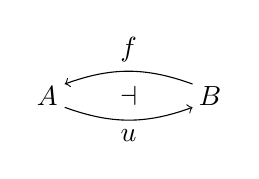
\begin{tikzpicture}[x=1.4em,y=1.4em]
  \node (A) at (0,0) {$A$};
  \node (B) at (4.2,0) {$B$};
  \draw[->] (3.75,0.3) to[bend right=20] node[above]{$f$} (0.45,0.3);
  \node at (2.1,0) {$\dashv$};
  \draw[->] (0.45,-0.3) to[bend right=20] node[below]{$u$} (3.75,-0.3);
\end{tikzpicture}
\end{center}
\begin{enumerate}[label=(\roman*)]
\item 对任何\trInfinityCategory $X$，
\begin{center}
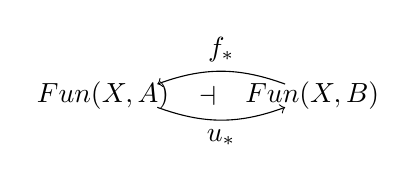
\begin{tikzpicture}[x=1.4em,y=1.4em]
  \node (A) at (0,0) {$\Fun(X,A)$};
  \node (B) at (5.4,0) {$\Fun(X,B)$};
  \draw[->] (4.7,0.3) to[bend right=20] node[above]{$f_\ast$} (1.4,0.3);
  \node at (2.7,0) {$\dashv$};
  \draw[->] (1.4,-0.3) to[bend right=20] node[below]{$u_\ast$} (4.7,-0.3);
\end{tikzpicture}
\end{center}
定义了\trQuasiCategory{}之间的一个\trAdjunction{}；
\item 对任何\trInfinityCategory $X$，
\begin{center}
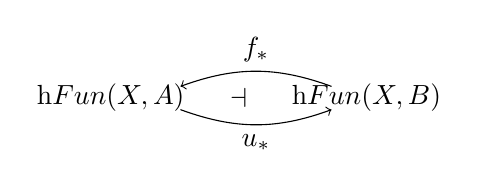
\begin{tikzpicture}[x=1.4em,y=1.4em]
  \node (A) at (0,0) {$\mathrm{h}\Fun(X,A)$};
  \node (B) at (6.6,0) {$\mathrm{h}\Fun(X,B)$};
  \draw[->] (5.7,0.3) to[bend right=20] node[above]{$f_\ast$} (1.8,0.3);
  \node at (3.3,0) {$\dashv$};
  \draw[->] (1.8,-0.3) to[bend right=20] node[below]{$u_\ast$} (5.7,-0.3);
\end{tikzpicture}
\end{center}
定义了\trCategory{}之间的一个\trAdjunction{}；
\item 对任何\trSimplicialSet $U$，
\begin{center}
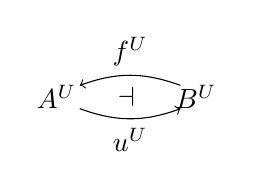
\begin{tikzpicture}[x=1.4em,y=1.4em]
  \node (A) at (0,0) {$A^{U}$};
  \node (B) at (3.6,0) {$B^{U}$};
  \draw[->] (3.2,0.3) to[bend right=20] node[above]{$f^{U}$} (0.6,0.3);
  \node at (1.8,0) {$\dashv$};
  \draw[->] (0.6,-0.3) to[bend right=20] node[below]{$u^{U}$} (3.2,-0.3);
\end{tikzpicture}
\end{center}
定义了\trInfinityCategory{}之间的一个\trAdjunction{}；而且
\item 若周围\trInfinityCosmos{}是\trCartesianClosed{}，则对任何%
\trInfinityCategory $C$，
\begin{center}
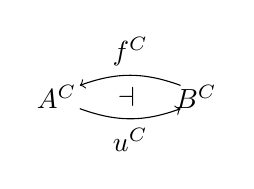
\begin{tikzpicture}[x=1.4em,y=1.4em]
  \node (A) at (0,0) {$A^{C}$};
  \node (B) at (3.6,0) {$B^{C}$};
  \draw[->] (3.2,0.3) to[bend right=20] node[above]{$f^{C}$} (0.6,0.3);
  \node at (1.8,0) {$\dashv$};
  \draw[->] (0.6,-0.3) to[bend right=20] node[below]{$u^{C}$} (3.2,-0.3);
\end{tikzpicture}
\end{center}
定义了\trInfinityCategory{}之间的一个\trAdjunction{}。
\end{enumerate}
\end{proposition}

例如，在 (ii) 中取 $X=1$，便得到\trInfinityCategory $A$ 与 $B$ 的%
\trHomotopyCategory{}之间的一个「导出」\trAdjunction{}（见定义 1.4.11）：
\begin{center}
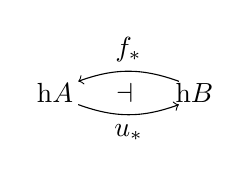
\begin{tikzpicture}[x=1.4em,y=1.4em]
  \node (A) at (0,0) {$\mathrm{h}A$};
  \node (B) at (3.6,0) {$\mathrm{h}B$};
  \draw[->] (3.2,0.3) to[bend right=20] node[above]{$f_\ast$} (0.6,0.3);
  \node at (1.8,0) {$\dashv$};
  \draw[->] (0.6,-0.3) to[bend right=20] node[below]{$u_\ast$} (3.2,-0.3);
\end{tikzpicture}
\end{center}
\begin{proof}
\trHomotopyTwoCategory{} $\mathrm{h}\mathcal{K}$ 的任何\trAdjunction
$f\dashv u$ 都被下列\trTwoFunctor{}保持：
$\Fun(X,-)\colon\mathrm{h}\mathcal{K}\to\mathrm{h}\QCat$、
$\mathrm{h}\Fun(X,-)\colon\mathrm{h}\mathcal{K}\to\Cat$、
$(-)^{U}\colon\mathrm{h}\mathcal{K}\to\mathrm{h}\mathcal{K}$ 与
$(-)^{C}\colon\mathrm{h}\mathcal{K}\to\mathrm{h}\mathcal{K}$。
\end{proof}

\begin{remark}\label{rem:contravariant-adjunction-preservation}
\cref{prop:adjunction-preservation}的每条\trAdjunction{}保持结果都有反变版本；
我们在此详解其中第一条（进一步的讨论见\cref{ex:cotensor-2-functor}）。把%
\trFunctorSpace{}的余域变元固定在任意\trInfinityCategory{} $C\in\mathcal{K}$ 上，
便定义了一个\trTwoFunctor
\[
\Fun(-,C)\colon\mathcal{K}^{op}\longrightarrow\mathrm{h}\QCat
\]
它在 1-\trCell{}上反变而在 2-\trCell{}上共变。\footnote{在 2-\trCategory{}上，
上标「op」表示 1-\trCell{}反转而 2-\trCell{}不反转；上标「co」表示 2-\trCell{}%
反转而 1-\trCell{}不反转；上标「coop」表示 1-\trCell{}与 2-\trCell{}皆反转
（见附录 B 中的\cref{def:op-co-duals}）。%
}这类\trTwoFunctor{}保持\trAdjunction{}，但交换左、\trRightAdjoint{}：比如，给定 $\mathcal{K}$
中的 $f\dashv u$，我们便得到\trFunctorSpace{}之间的一个\trAdjunction{}
\begin{center}
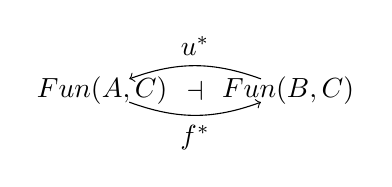
\begin{tikzpicture}[x=1.4em,y=1.4em]
  \node (A) at (0,0) {$\Fun(A,C)$};
  \node (B) at (4.8,0) {$\Fun(B,C)$};
  \draw[->] (4.1,0.3) to[bend right=20] node[above]{$u^{\ast}$} (0.7,0.3);
  \node at (2.4,0) {$\dashv$};
  \draw[->] (0.7,-0.3) to[bend right=20] node[below]{$f^{\ast}$} (4.1,-0.3);
\end{tikzpicture}
\end{center}
\end{remark}

接下来的五个结果都有标准证明，随时可以「现货取用」——只需向恰好驻足近旁的
任意一位 2-范畴理论家讨教即可。唯一的新意在于指出：这些标准论证可以应用到%
\trInfinityCategory{}之间的\trAdjunction{}理论上。

\begin{proposition}\label{prop:adjunctions-compose}
\trAdjunction{}可合成：给定伴随\trFunctor
\begin{center}
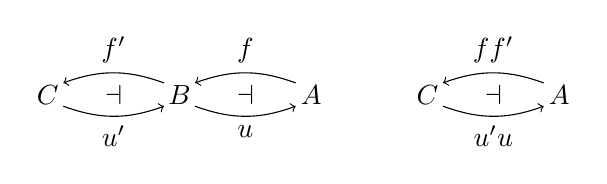
\begin{tikzpicture}[x=1.4em,y=1.4em]
  \node (C) at (0,0) {$C$};
  \node (B) at (3.4,0) {$B$};
  \node (A) at (6.8,0) {$A$};
  \draw[->] (3.0,0.3) to[bend right=20] node[above]{$f'$} (0.4,0.3);
  \node at (1.7,0) {$\dashv$};
  \draw[->] (0.4,-0.3) to[bend right=20] node[below]{$u'$} (3.0,-0.3);
  \draw[->] (6.4,0.3) to[bend right=20] node[above]{$f$} (3.8,0.3);
  \node at (5.1,0) {$\dashv$};
  \draw[->] (3.8,-0.3) to[bend right=20] node[below]{$u$} (6.4,-0.3);
  \node at (8.3,0) {$\rightsquigarrow$};
  \node (C2) at (9.8,0) {$C$};
  \node (A2) at (13.2,0) {$A$};
  \draw[->] (12.8,0.3) to[bend right=20] node[above]{$ff'$} (10.2,0.3);
  \node at (11.5,0) {$\dashv$};
  \draw[->] (10.2,-0.3) to[bend right=20] node[below]{$u'u$} (12.8,-0.3);
\end{tikzpicture}
\end{center}
则复合\trFunctor{}是伴随的。
\end{proposition}
\begin{proof}
记 $\eta\colon\mathrm{id}_B\Rightarrow uf$、$\epsilon\colon fu\Rightarrow\mathrm{id}_A$、
$\eta'\colon\mathrm{id}_C\Rightarrow u'f'$ 与
$\epsilon'\colon f'u'\Rightarrow\mathrm{id}_B$ 为各自的\trUnit{}与\trCounit{}，则粘贴图
\begin{center}
\begin{tikzpicture}[x=1.35em,y=1.35em]
  \node (C1) at (0,2.9) {$C$};
  \node (C2) at (3.6,2.9) {$C$};
  \node (B1) at (1.8,1.45) {$B$};
  \node (B2) at (5.4,1.45) {$B$};
  \node (Ac) at (3.6,0) {$A$};
  \draw[double] (0.42,2.9) -- (3.18,2.9);
  \draw[double] (2.22,1.45) -- (4.98,1.45);
  \draw[->] (0.32,2.66) -- (1.5,1.69);
  \node at (0.35,2.3) {$f'$};
  \draw[->] (2.1,1.69) -- (3.28,2.66);
  \node at (2.35,2.35) {$u'$};
  \draw[->] (2.1,1.2) -- (3.3,0.24);
  \node at (2.0,0.62) {$f$};
  \draw[->] (3.9,0.24) -- (5.08,1.2);
  \node at (5.35,0.62) {$u$};
  \node at (1.8,2.42) {$\scriptstyle\Downarrow\eta'$};
  \node at (3.6,0.97) {$\scriptstyle\Downarrow\eta$};
  \node at (6.0,1.45) {及};
  \node (C3) at (9.2,2.9) {$C$};
  \node (B3) at (7.9,1.45) {$B$};
  \node (B4) at (11.5,1.45) {$B$};
  \node (A3) at (6.7,0) {$A$};
  \node (A4) at (10.3,0) {$A$};
  \draw[double] (8.32,1.45) -- (11.08,1.45);
  \draw[double] (7.12,0) -- (9.88,0);
  \draw[->] (8.22,1.69) -- (8.98,2.66);
  \node at (7.8,2.3) {$u'$};
  \draw[->] (9.42,2.66) -- (10.58,1.69);
  \node at (10.6,2.3) {$f'$};
  \draw[->] (6.92,0.22) -- (7.68,1.21);
  \node at (6.65,0.75) {$u$};
  \draw[->] (8.22,1.21) -- (9.98,0.24);
  \node at (10.1,0.55) {$f$};
  \node at (9.2,1.95) {$\scriptstyle\Downarrow\epsilon'$};
  \node at (8.35,0.5) {$\scriptstyle\Downarrow\epsilon$};
\end{tikzpicture}
\end{center}
定义了 $ff'\dashv u'u$ 的\trUnit{}与\trCounit{}，使得\trTriangleEqualities{}成立：
\begin{center}
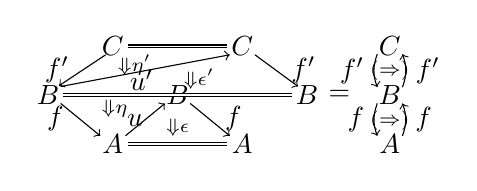
\begin{tikzpicture}[x=1.3em,y=1.22em]
  \node (C1) at (0,4.35) {$C$};
  \node (C2) at (3.6,4.35) {$C$};
  \node (B1) at (-1.8,2.9) {$B$};
  \node (B2) at (1.8,2.9) {$B$};
  \node (B3) at (5.4,2.9) {$B$};
  \node (A1) at (0,1.45) {$A$};
  \node (A2) at (3.6,1.45) {$A$};
  \draw[double] (0.42,4.35) -- (3.18,4.35);
  \draw[double] (-1.38,2.9) -- (4.98,2.9);
  \draw[double] (0.42,1.45) -- (3.18,1.45);
  \draw[->] (-0.2,4.1) -- (-1.5,3.18);
  \node at (-1.55,3.65) {$f'$};
  \draw[->] (-1.45,3.16) -- (3.25,4.1);
  \node at (0.8,3.35) {$u'$};
  \draw[->] (3.95,4.1) -- (5.15,3.16);
  \node at (5.3,3.65) {$f'$};
  \draw[->] (-1.45,2.66) -- (-0.35,1.7);
  \node at (-1.6,2.2) {$f$};
  \draw[->] (0.35,1.7) -- (1.45,2.66);
  \node at (0.62,2.14) {$u$};
  \draw[->] (2.15,2.66) -- (3.25,1.7);
  \node at (3.35,2.2) {$f$};
  \node at (0.6,3.8) {$\scriptstyle\Downarrow\eta'$};
  \node at (2.4,3.38) {$\scriptstyle\Downarrow\epsilon'$};
  \node at (0.05,2.5) {$\scriptstyle\Downarrow\eta$};
  \node at (1.8,1.93) {$\scriptstyle\Downarrow\epsilon$};
  \node at (6.3,2.9) {$=$};
  \node (Cs) at (7.7,4.35) {$C$};
  \node (Bs) at (7.7,2.9) {$B$};
  \node (As) at (7.7,1.45) {$A$};
  \draw[->] (7.35,4.12) to[bend right=20] node[left]{$f'$} (7.35,3.14);
  \draw[->] (8.05,3.14) to[bend right=20] node[right]{$f'$} (8.05,4.12);
  \node at (7.7,3.62) {$\scriptstyle(\Rightarrow)$};
  \draw[->] (7.35,2.66) to[bend right=20] node[left]{$f$} (7.35,1.7);
  \draw[->] (8.05,1.7) to[bend right=20] node[right]{$f$} (8.05,2.66);
  \node at (7.7,2.16) {$\scriptstyle(\Rightarrow)$};
\end{tikzpicture}
\end{center}
\begin{center}
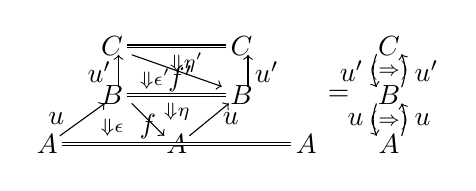
\begin{tikzpicture}[x=1.3em,y=1.22em]
  \node (C1) at (0,4.35) {$C$};
  \node (C2) at (3.6,4.35) {$C$};
  \node (B1) at (0,2.9) {$B$};
  \node (B2) at (3.6,2.9) {$B$};
  \node (A1) at (-1.8,1.45) {$A$};
  \node (A2) at (1.8,1.45) {$A$};
  \node (A3) at (5.4,1.45) {$A$};
  \draw[double] (0.42,4.35) -- (3.18,4.35);
  \draw[double] (0.42,2.9) -- (3.18,2.9);
  \draw[double] (-1.38,1.45) -- (4.98,1.45);
  \draw[->] (0.18,3.14) -- (0.18,4.1);
  \node at (-0.35,3.6) {$u'$};
  \draw[->] (0.55,4.1) -- (3.05,3.16);
  \node at (1.9,3.4) {$f'$};
  \draw[->] (3.78,3.14) -- (3.78,4.1);
  \node at (4.3,3.6) {$u'$};
  \draw[->] (-1.45,1.7) -- (-0.2,2.66);
  \node at (-1.55,2.2) {$u$};
  \draw[->] (0.55,2.66) -- (1.45,1.7);
  \node at (1.0,1.98) {$f$};
  \draw[->] (2.15,1.7) -- (3.25,2.66);
  \node at (3.3,2.2) {$u$};
  \node at (1.2,3.38) {$\scriptstyle\Downarrow\epsilon'$};
  \node at (2.07,3.87) {$\scriptstyle\Downarrow\eta'$};
  \node at (0.0,1.93) {$\scriptstyle\Downarrow\epsilon$};
  \node at (1.8,2.42) {$\scriptstyle\Downarrow\eta$};
  \node at (6.3,2.9) {$=$};
  \node (Cs) at (7.7,4.35) {$C$};
  \node (Bs) at (7.7,2.9) {$B$};
  \node (As) at (7.7,1.45) {$A$};
  \draw[->] (7.35,4.12) to[bend right=20] node[left]{$u'$} (7.35,3.14);
  \draw[->] (8.05,3.14) to[bend right=20] node[right]{$u'$} (8.05,4.12);
  \node at (7.7,3.62) {$\scriptstyle(\Rightarrow)$};
  \draw[->] (7.35,2.66) to[bend right=20] node[left]{$u$} (7.35,1.7);
  \draw[->] (8.05,1.7) to[bend right=20] node[right]{$u$} (8.05,2.66);
  \node at (7.7,2.16) {$\scriptstyle(\Rightarrow)$};
\end{tikzpicture}
\end{center}
\end{proof}

给定\trFunctor{}的伴随在同构意义下唯一：

\begin{proposition}[伴随的唯一性]\label{prop:uniqueness-of-adjoints}
\begin{enumerate}[label=(\roman*)]
\item 若 $f\dashv u$ 且 $f'\dashv u$，则 $f\cong f'$。
\item 反之，若 $f\dashv u$ 且 $f\cong f'$，则 $f'\dashv u$。
\end{enumerate}
\end{proposition}
\begin{proof}
记 $\eta\colon\mathrm{id}_B\Rightarrow uf$、$\epsilon\colon fu\Rightarrow\mathrm{id}_A$、
$\eta'\colon\mathrm{id}_B\Rightarrow uf'$ 与
$\epsilon'\colon f'u\Rightarrow\mathrm{id}_A$ 为各自的\trUnit{}与\trCounit{}，则粘贴图
\begin{center}
\begin{tikzpicture}[x=1.35em,y=1.35em]
  \node (B1) at (0,1.5) {$B$};
  \node (B2) at (3.6,1.5) {$B$};
  \node (A1) at (1.8,0) {$A$};
  \node (A2) at (5.4,0) {$A$};
  \draw[double] (0.42,1.5) -- (3.18,1.5);
  \draw[double] (2.22,0) -- (4.98,0);
  \draw[->] (0.32,1.26) -- (1.52,0.22);
  \node at (0.45,0.75) {$f'$};
  \draw[->] (2.12,0.22) -- (3.28,1.26);
  \node at (3.0,0.4) {$u$};
  \draw[->] (3.92,1.26) -- (5.08,0.22);
  \node at (5.15,0.75) {$f$};
  \node at (1.8,1.0) {$\scriptstyle\Downarrow\eta'$};
  \node at (3.75,0.62) {$\scriptstyle\Downarrow\epsilon$};
  \node at (6.6,0.75) {与};
  \node (B3) at (7.5,1.5) {$B$};
  \node (B4) at (11.1,1.5) {$B$};
  \node (A3) at (9.3,0) {$A$};
  \node (A4) at (12.9,0) {$A$};
  \draw[double] (7.92,1.5) -- (10.68,1.5);
  \draw[double] (9.72,0) -- (12.48,0);
  \draw[->] (7.82,1.26) -- (9.02,0.22);
  \node at (7.95,0.75) {$f$};
  \draw[->] (9.62,0.22) -- (10.78,1.26);
  \node at (10.5,0.4) {$u$};
  \draw[->] (11.42,1.26) -- (12.62,0.22);
  \node at (12.75,0.6) {$f'$};
  \node at (9.3,1.0) {$\scriptstyle\Downarrow\eta$};
  \node at (11.25,0.62) {$\scriptstyle\Downarrow\epsilon'$};
\end{tikzpicture}
\end{center}
定义了 2-\trCell{} $f\Rightarrow f'$ 与 $f'\Rightarrow f$。复合
$f\Rightarrow f'\Rightarrow f$ 与 $f'\Rightarrow f\Rightarrow f'$ 则通过把这两张图
从某一侧或另一侧水平地粘贴起来而计算。对\trAdjunction{} $f\dashv u$ 与
$f'\dashv u$ 应用\trTriangleEqualities{}，易见这两个复合都是恒等。于是作为从 $B$ 到 $A$ 的%
\trFunctor{}有 $f\cong f'$。

(ii) 留作\cref{ex:uniqueness-converse}。
\end{proof}

下面的结果削弱了\cref{def:adjunction}的假设。

\begin{lemma}[最小伴随数据]\label{lem:minimal-adjunction-data}
一对\trFunctor{} $f\colon B\to A$ 与 $u\colon A\to B$ 构成伴随对 $f\dashv u$，
当且仅当存在\trNaturalTransformation{} $\mathrm{id}_B\Rightarrow uf$ 与
$fu\Rightarrow\mathrm{id}_A$，使得\trTriangleEqualities{}复合
$f\Rightarrow fuf\Rightarrow f$ 与 $u\Rightarrow ufu\Rightarrow u$ 皆可逆。
\end{lemma}
\begin{proof}
一个\trAdjunction{}的\trUnit{}与\trCounit{}当然满足这些假设。反之，设
$\eta\colon\mathrm{id}_B\Rightarrow uf$ 与 $\epsilon'\colon fu\Rightarrow\mathrm{id}_A$
是这样一对\trNaturalTransformation{}，使得\trTriangleEqualities{}复合
\[
\phi\coloneqq f\xrightarrow{\;f\eta\;}fuf\xrightarrow{\;\epsilon' f\;}f
\qquad\qquad
\psi\coloneqq u\xrightarrow{\;\eta u\;}ufu\xrightarrow{\;u\epsilon'\;}u
\]
是同构。我们要构造一个以 $\eta$ 为\trUnit{}的\trAdjunction{} $f\dashv u$，办法是把
$\epsilon'$ 修改成\trCounit $\epsilon$。\footnote{由这一构造的余对偶，也可以改为取
$\epsilon'$ 作\trCounit{}，而代价是修改 $\eta$ 来形成\trUnit
（见\cref{ex:dual-minimal-data}）。}为解释这一构造的想法，注意：对一对取定的\trGeneralizedElement
$b\colon X\to B$ 与 $a\colon X\to A$，与 $\eta$ 及 $\epsilon'$ 作粘贴便在所示诸%
\trNaturalTransformation{}之集之间定义了若干函数：
\begin{center}
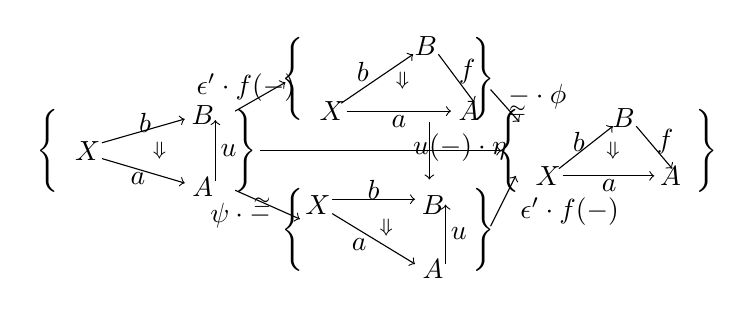
\begin{tikzpicture}[x=1.3em,y=1.3em]
  \begin{scope}[shift={(0,3.2)}]
    \node at (-2.6,0) {$\Bigg\{$};
    \node at (2.9,0) {$\Bigg\}$};
    \node (XL) at (-1.5,0) {$X$};
    \node (BL) at (1.7,1.0) {$B$};
    \node (AL) at (1.7,-1.0) {$A$};
    \draw[->] (-1.1,0.22) -- (1.2,0.88);
    \node at (0.1,0.78) {$b$};
    \draw[->] (-1.1,-0.22) -- (1.2,-0.9);
    \node at (-0.1,-0.78) {$a$};
    \draw[->] (2.05,-0.85) -- (2.05,0.85);
    \node at (2.42,0) {$u$};
    \node at (0.5,0.0) {$\scriptstyle\Downarrow$};
  \end{scope}
  \begin{scope}[shift={(6.4,5.2)}]
    \node at (-2.2,0) {$\Bigg\{$};
    \node at (3.1,0) {$\Bigg\}$};
    \node (XT) at (-1.1,-0.9) {$X$};
    \node (BT) at (1.5,0.9) {$B$};
    \node (AT) at (2.7,-0.9) {$A$};
    \draw[->] (-0.85,-0.68) -- (1.15,0.68);
    \node at (-0.25,0.2) {$b$};
    \draw[->] (1.85,0.68) -- (2.85,-0.66);
    \node at (2.65,0.2) {$f$};
    \draw[->] (-0.7,-0.9) -- (2.2,-0.9);
    \node at (0.75,-1.18) {$a$};
    \node at (0.85,-0.05) {$\scriptstyle\Downarrow$};
  \end{scope}
  \begin{scope}[shift={(6.4,1.0)}]
    \node at (-2.2,0) {$\Bigg\{$};
    \node at (3.1,0) {$\Bigg\}$};
    \node (XB) at (-1.5,0.7) {$X$};
    \node (BB) at (1.7,0.7) {$B$};
    \node (AB) at (1.7,-1.1) {$A$};
    \draw[->] (-1.1,0.85) -- (1.2,0.85);
    \node at (0.05,1.12) {$b$};
    \draw[->] (-1.1,0.45) -- (1.2,-0.95);
    \node at (-0.35,-0.42) {$a$};
    \draw[->] (2.05,-0.95) -- (2.05,0.7);
    \node at (2.42,-0.1) {$u$};
    \node at (0.4,0.05) {$\scriptstyle\Downarrow$};
  \end{scope}
  \begin{scope}[shift={(12.8,3.2)}]
    \node at (-2.6,0) {$\Bigg\{$};
    \node at (2.9,0) {$\Bigg\}$};
    \node (XR) at (-1.5,-0.7) {$X$};
    \node (BR) at (0.6,0.9) {$B$};
    \node (AR) at (1.9,-0.7) {$A$};
    \draw[->] (-1.2,-0.5) -- (0.3,0.68);
    \node at (-0.65,0.25) {$b$};
    \draw[->] (0.95,0.68) -- (1.95,-0.5);
    \node at (1.75,0.25) {$f$};
    \draw[->] (-1.1,-0.7) -- (1.45,-0.7);
    \node at (0.2,-0.98) {$a$};
    \node at (0.3,0.0) {$\scriptstyle\Downarrow$};
  \end{scope}
  \draw[->] (2.6,4.3) -- (4.0,5.1);
  \node at (2.9,4.95) {$\epsilon'\cdot f(-)$};
  \draw[->] (9.7,4.9) -- (10.5,4.0);
  \node at (11.0,4.7) {$-\cdot\phi$};
  \node at (10.45,4.3) {$\scriptstyle\simeq$};
  \draw[->] (2.6,2.1) -- (4.4,1.3);
  \node at (2.75,1.4) {$\psi\cdot-$};
  \node at (3.35,1.75) {$\scriptstyle\simeq$};
  \draw[->] (9.7,1.1) -- (10.4,2.5);
  \node at (11.9,1.5) {$\epsilon'\cdot f(-)$};
  \draw[->] (8.0,4.0) -- (8.0,2.4);
  \node at (8.85,3.3) {$u(-)\cdot\eta$};
  \draw[->] (3.3,3.2) -- (10.0,3.2);
\end{tikzpicture}
\end{center}
由「\trTriangleEqualities{}复合是同构」这一假设，这些函数中有两个可逆，再由\trIsomorphism{}的%
\trTwoOfSixProperty{}，全部六个映射都是双射。
定义「修正过的」\trCounit{}为如下复合：
\begin{center}
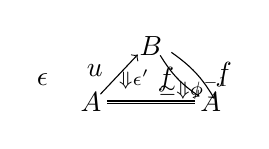
\begin{tikzpicture}[x=1.35em,y=1.35em]
  \node at (-2.9,0.6) {$\epsilon\coloneqq$};
  \node (Bc) at (0,1.5) {$B$};
  \node (A1c) at (-1.6,0) {$A$};
  \node (A2c) at (1.6,0) {$A$};
  \draw[double] (-1.18,0) -- (1.18,0);
  \draw[->] (-1.35,0.22) -- (-0.35,1.28);
  \node at (-1.5,0.85) {$u$};
  \draw[->] (0.25,1.26) to[bend right=12] (1.3,0.16);
  \node at (0.4,0.6) {$f$};
  \draw[->] (0.55,1.34) to[bend left=12] (1.7,0.1);
  \node at (1.95,0.75) {$f$};
  \node at (-0.45,0.62) {$\scriptstyle\Downarrow\epsilon'$};
  \node at (1.15,0.38) {$\scriptstyle\simeq\Downarrow\phi^{-1}$};
\end{tikzpicture}
\end{center}
使得\trTriangleEqualities{}复合之一约化为恒等：
\begin{center}
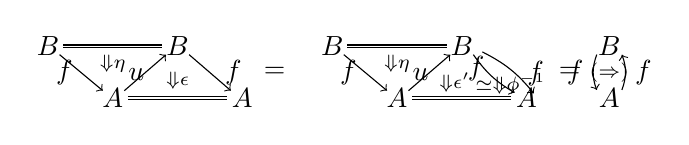
\begin{tikzpicture}[x=1.3em,y=1.25em]
  \node (B1) at (0,1.5) {$B$};
  \node (B2) at (3.6,1.5) {$B$};
  \node (A1) at (1.8,0) {$A$};
  \node (A2) at (5.4,0) {$A$};
  \draw[double] (0.42,1.5) -- (3.18,1.5);
  \draw[double] (2.22,0) -- (4.98,0);
  \draw[->] (0.32,1.26) -- (1.52,0.22);
  \node at (0.45,0.75) {$f$};
  \draw[->] (2.12,0.22) -- (3.28,1.26);
  \node at (2.45,0.68) {$u$};
  \draw[->] (3.92,1.26) -- (5.08,0.22);
  \node at (5.15,0.75) {$f$};
  \node at (1.8,1.0) {$\scriptstyle\Downarrow\eta$};
  \node at (3.6,0.5) {$\scriptstyle\Downarrow\epsilon$};
  \node at (6.3,0.75) {$=$};
  \node (B3) at (7.9,1.5) {$B$};
  \node (B4) at (11.5,1.5) {$B$};
  \node (A3) at (9.7,0) {$A$};
  \node (A4) at (13.3,0) {$A$};
  \draw[double] (8.32,1.5) -- (11.08,1.5);
  \draw[double] (10.12,0) -- (12.88,0);
  \draw[->] (8.22,1.26) -- (9.42,0.22);
  \node at (8.35,0.75) {$f$};
  \draw[->] (10.02,0.22) -- (11.18,1.26);
  \node at (10.35,0.68) {$u$};
  \draw[->] (11.82,1.26) to[bend right=12] (12.97,0.16);
  \node at (11.9,0.85) {$f$};
  \draw[->] (12.07,1.34) to[bend left=12] (13.5,0.14);
  \node at (13.55,0.7) {$f$};
  \node at (9.7,1.0) {$\scriptstyle\Downarrow\eta$};
  \node at (11.3,0.45) {$\scriptstyle\Downarrow\epsilon'$};
  \node at (12.85,0.42) {$\scriptstyle\simeq\Downarrow\phi^{-1}$};
  \node at (14.5,0.75) {$=$};
  \node (Bt) at (15.6,1.5) {$B$};
  \node (At) at (15.6,0) {$A$};
  \draw[->] (15.25,1.26) to[bend right=20] node[left]{$f$} (15.25,0.24);
  \draw[->] (15.95,0.24) to[bend right=20] node[right]{$f$} (15.95,1.26);
  \node at (15.6,0.75) {$\scriptstyle(\Rightarrow)$};
\end{tikzpicture}
\end{center}
现在由粘贴等式
\begin{center}
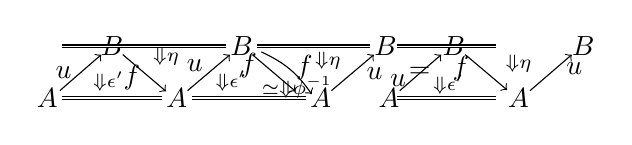
\begin{tikzpicture}[x=1.3em,y=1.25em]
  \node (B1) at (0,1.5) {$B$};
  \node (B2) at (3.6,1.5) {$B$};
  \node (B3) at (7.6,1.5) {$B$};
  \node (A1) at (-1.8,0) {$A$};
  \node (A2) at (1.8,0) {$A$};
  \node (A3) at (5.8,0) {$A$};
  \draw[double] (-1.38,1.5) -- (3.18,1.5);
  \draw[double] (4.02,1.5) -- (7.18,1.5);
  \draw[double] (-1.38,0) -- (1.38,0);
  \draw[double] (2.22,0) -- (5.38,0);
  \draw[->] (-1.45,0.22) -- (-0.3,1.26);
  \node at (-1.35,0.75) {$u$};
  \draw[->] (0.3,1.26) -- (1.5,0.2);
  \node at (0.55,0.6) {$f$};
  \draw[->] (2.1,0.22) -- (3.28,1.26);
  \node at (2.3,0.95) {$u$};
  \draw[->] (3.9,1.26) -- (5.1,0.2);
  \node at (3.8,0.95) {$f$};
  \draw[->] (4.15,1.34) to[bend left=15] (5.55,0.12);
  \node at (5.35,0.9) {$f$};
  \draw[->] (6.1,0.22) -- (7.28,1.26);
  \node at (7.3,0.7) {$u$};
  \node at (-0.1,0.48) {$\scriptstyle\Downarrow\epsilon'$};
  \node at (1.5,1.2) {$\scriptstyle\Downarrow\eta$};
  \node at (3.3,0.5) {$\scriptstyle\Downarrow\epsilon'$};
  \node at (5.14,0.32) {$\scriptstyle\simeq\Downarrow\phi^{-1}$};
  \node at (6.0,1.1) {$\scriptstyle\Downarrow\eta$};
  \node at (8.55,0.75) {$=$};
  \node (B4) at (9.5,1.5) {$B$};
  \node (B5) at (13.1,1.5) {$B$};
  \node (A4) at (7.7,0) {$A$};
  \node (A5) at (11.3,0) {$A$};
  \draw[double] (7.92,1.5) -- (10.68,1.5);
  \draw[double] (7.92,0) -- (10.68,0);
  \draw[->] (8.0,0.22) -- (9.15,1.26);
  \node at (7.95,0.5) {$u$};
  \draw[->] (9.82,1.26) -- (10.98,0.24);
  \node at (9.7,0.85) {$f$};
  \draw[->] (11.62,0.22) -- (12.78,1.26);
  \node at (12.85,0.85) {$u$};
  \node at (9.35,0.4) {$\scriptstyle\Downarrow\epsilon'$};
  \node at (11.3,1.0) {$\scriptstyle\Downarrow\eta$};
\end{tikzpicture}
\end{center}
我们看到 $(u\epsilon\cdot\eta u)\cdot\psi=\psi$。由于 $\psi$ 可逆，可以消去，从而
得出 $u\epsilon\cdot\eta u=\mathrm{id}_u$。
\end{proof}

2-范畴论中有一个标准结果：2-\trCategory{}中的任何\trEquivalence{}都可以被提升为
一个同时还定义\trAdjunction{}的\trEquivalence{}：

\begin{proposition}[\trAdjointEquivalence]\label{prop:adjoint-equivalences}

任何\trEquivalence{}都可以通过修改其中一个 2-\trCell{}而被提升为一个\textbf{\trAdjointEquivalence}
（adjoint equivalence）。也就是说，可以如此选取\trEquivalence{}中的诸可逆
2-\trCell{}，使之满足\trTriangleEqualities{}。因此，若 $f$ 与 $g$ 是互逆的\trEquivalence{}，
则 $f\dashv g$ 且 $g\dashv f$。
\end{proposition}
\begin{proof}
考虑一个由\trFunctor{} $f\colon A\to B$ 与 $g\colon B\to A$ 连同可逆 2-\trCell{}
\begin{center}
\begin{tikzpicture}[x=1.35em,y=1.35em]
  \node (A1) at (0,0) {$A$};
  \node (A2) at (2.6,0) {$A$};
  \draw[double] (0.4,0.14) -- (2.2,0.14);
  \draw[->] (0.4,-0.18) to[bend right=25] node[below]{$gf$} (2.2,-0.18);
  \node at (1.3,-0.15) {$\scriptstyle\simeq\Downarrow\alpha$};   %
  \node at (4.1,0) {及};
  \node (B1) at (5.6,0) {$B$};
  \node (B2) at (8.2,0) {$B$};
  \draw[->] (6.0,0.18) to[bend left=25] node[above]{$fg$} (7.8,0.18);
  \draw[double] (6.0,-0.14) -- (7.8,-0.14);
  \node at (6.9,0.12) {$\scriptstyle\simeq\Downarrow\beta$};   %
\end{tikzpicture}
\end{center}
构成的一个\trEquivalence{}。由于 $\alpha$ 与 $\beta$ 皆可逆，\trTriangleEqualities{}复合亦然，
于是\cref{lem:minimal-adjunction-data}的构造适用。
\end{proof}

\cref{prop:adjoint-equivalences}的一个用途是证明：\trAdjunction{}在\trEquivalence{}%
之下不变：

\begin{proposition}\label{prop:adjunction-equivalence-invariant}
\trInfinityCategory{}之间的\trFunctor{} $u\colon A\to B$ 容许一个\trLeftAdjoint{}，当且仅当
对任意一对等价的\trInfinityCategory{} $A'\simeq A$ 与 $B'\simeq B$，与之等价的%
\trFunctor{} $u'\colon A'\to B'$ 容许一个\trLeftAdjoint{}。
\end{proposition}

我们将会发现，∞-\trCategory{}理论的整体在这种意义下都是\trEquivalence{}不变的。

\begin{proof}
若 $u\colon A\to B$ 容许一个\trLeftAdjoint{}，则把 $f\dashv u$ 与\trAdjointEquivalence
$A'\simeq A$ 及 $B\simeq B'$ 复合，便得到一个与之等价的\trAdjunction{}：
\begin{center}
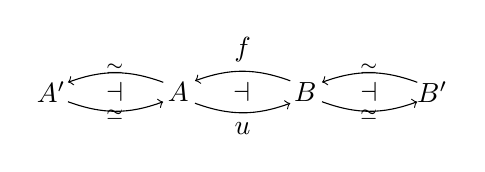
\begin{tikzpicture}[x=1.35em,y=1.35em]
  \node (Ap) at (0,0) {$A'$};
  \node (Am) at (3.4,0) {$A$};
  \node (Bm) at (6.8,0) {$B$};
  \node (Bp) at (10.2,0) {$B'$};
  \draw[->] (3.0,0.26) to[bend right=20] (0.45,0.26);
  \node at (1.7,0.62) {$\scriptstyle\simeq$};
  \node at (1.7,0) {$\dashv$};
  \draw[->] (0.45,-0.26) to[bend right=20] (3.0,-0.26);
  \node at (1.7,-0.62) {$\scriptstyle\simeq$};
  \draw[->] (6.4,0.3) to[bend right=20] node[above]{$f$} (3.85,0.3);
  \node at (5.1,0) {$\dashv$};
  \draw[->] (3.85,-0.3) to[bend right=20] node[below]{$u$} (6.4,-0.3);
  \draw[->] (9.8,0.26) to[bend right=20] (7.25,0.26);
  \node at (8.5,0.62) {$\scriptstyle\simeq$};
  \node at (8.5,0) {$\dashv$};
  \draw[->] (7.25,-0.26) to[bend right=20] (9.8,-0.26);
  \node at (8.5,-0.62) {$\scriptstyle\simeq$};
\end{tikzpicture}
\end{center}
反之，若与之等价的\trFunctor{} $u'\colon A'\simeq A\xrightarrow{\;u\;}B\simeq B'$
容许一个\trLeftAdjoint $f'$，则同样得到一个复合\trAdjunction{}
\begin{center}
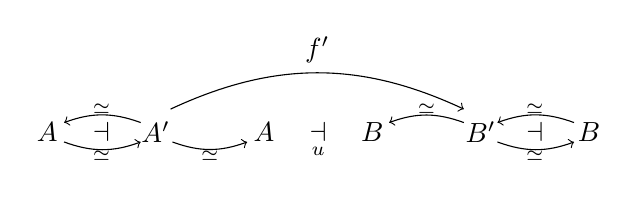
\begin{tikzpicture}[x=1.35em,y=1.35em]
  \node (Al) at (0,0) {$A$};
  \node (Ap) at (2.9,0) {$A'$};
  \node (Am) at (5.8,0) {$A$};
  \node (Bm) at (8.7,0) {$B$};
  \node (Bp) at (11.6,0) {$B'$};
  \node (Br) at (14.5,0) {$B$};
  \draw[->] (2.5,0.26) to[bend right=20] (0.45,0.26);
  \node at (1.45,0.62) {$\scriptstyle\simeq$};
  \node at (1.45,0) {$\dashv$};
  \draw[->] (0.45,-0.26) to[bend right=20] (2.5,-0.26);
  \node at (1.45,-0.62) {$\scriptstyle\simeq$};
  \draw[->] (3.35,-0.26) to[bend right=20] (5.35,-0.26);
  \node at (4.35,-0.62) {$\scriptstyle\simeq$};
  \node at (7.25,0) {$\dashv$};
  \node at (7.25,-0.5) {$\scriptstyle u$};
  \draw[->] (11.15,0.26) to[bend right=20] (9.15,0.26);
  \node at (10.15,0.62) {$\scriptstyle\simeq$};
  \draw[->] (14.1,0.26) to[bend right=20] (12.05,0.26);
  \node at (13.05,0.62) {$\scriptstyle\simeq$};
  \node at (13.05,0) {$\dashv$};
  \draw[->] (12.05,-0.26) to[bend right=20] (14.1,-0.26);
  \node at (13.05,-0.62) {$\scriptstyle\simeq$};
  \draw[->] (3.3,0.62) to[bend left=25] node[above]{$f'$} (11.15,0.62);
\end{tikzpicture}
\end{center}
其\trRightAdjoint{}与原先的\trFunctor{} $u$ 自然同构。于是由\cref{prop:uniqueness-of-adjoints}，
图中所示的\trLeftAdjoint{}就是 $u$ 的一个\trLeftAdjoint{}。
\end{proof}

为备后用，我们以一个抽象定义的\trAdjunction{}作结：经由本节证明的诸结果，它对
任何\trInfinityCosmos{}中的任何\trInfinityCategory{}都能构造出来。

\begin{lemma}\label{lem:composition-adjoint-triple}

对任何\trInfinityCategory{} $A$，「合成」函子
\begin{rveq}\label{eq:composition-functor}
\mbox{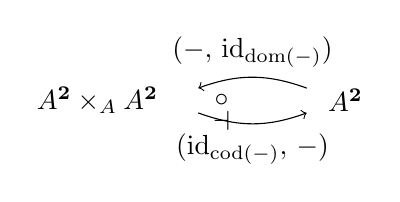
\begin{tikzpicture}[x=1.4em,y=1.4em]
  \node (L) at (0,0) {$A^{\qcTwo}\times_{A}A^{\qcTwo}$};
  \node (R) at (6.4,0) {$A^{\qcTwo}$};
  \draw[->] (5.4,0.32) to[bend right=20] node[above]
    {$(-,\,\mathrm{id}_{\mathrm{dom}(-)})$} (2.6,0.32);
  \node at (3.2,0) {$\circ$};
  \node at (3.2,-0.52) {$\dashv$};
  \draw[->] (2.6,-0.32) to[bend right=20] node[below]
    {$(\mathrm{id}_{\mathrm{cod}(-)},\,-)$} (5.4,-0.32);
\end{tikzpicture}}
\end{rveq}
容许左、右两个伴随，它们把一个箭头延拓成一个可合成的箭头对——分别通过让该箭头
与其定义域处或余域处的恒等箭头配对。
\end{lemma}
\begin{proof}
在 $\Delta\subset\Cat$ 中有一份对偶伴随（dual adjunction）数据，其诸\trFunctor{}%
可用 1.1.1 中引入的单纯算子记号描述：
\begin{center}
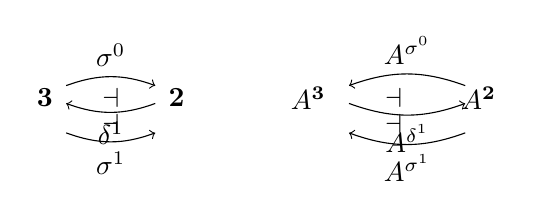
\begin{tikzpicture}[x=1.4em,y=1.4em]
  \node (T1) at (0,0) {$\qcThree$};
  \node (T2) at (3.4,0) {$\qcTwo$};
  \draw[->] (0.55,0.32) to[bend left=20] node[above]{$\sigma^{0}$} (2.85,0.32);
  \node at (1.7,0) {$\dashv$};
  \draw[->] (2.85,-0.14) to[bend left=20] node[below]{$\delta^{1}$} (0.55,-0.14);
  \node at (1.7,-0.66) {$\dashv$};
  \draw[->] (0.55,-0.9) to[bend right=20] node[below]{$\sigma^{1}$} (2.85,-0.9);
  \node at (5.1,0) {$\rightsquigarrow$};
  \node (T3) at (6.8,0) {$A^{\qcThree}$};
  \node (T4) at (11.2,0) {$A^{\qcTwo}$};
  \draw[->] (10.85,0.32) to[bend right=20] node[above]{$A^{\sigma^{0}}$} (7.85,0.32);
  \node at (9.0,0) {$\dashv$};
  \draw[->] (7.85,-0.14) to[bend right=20] node[below]{$A^{\delta^{1}}$} (10.85,-0.14);
  \node at (9.0,-0.66) {$\dashv$};
  \draw[->] (10.85,-0.9) to[bend left=20] node[below]{$A^{\sigma^{1}}$} (7.85,-0.9);
\end{tikzpicture}
\end{center}
对\trInfinityCosmos{} $\mathcal{K}$ 中的任何\trInfinityCategory{} $A$，
\cref{ex:cotensor-2-functor}描述了一个\trTwoFunctor{}
$A^{(-)}\colon\Cat^{op}\to\mathrm{h}\mathcal{K}$，它把上左所示的\trAdjointTriple{}搬运为
上右所示者。

现在我们断言：存在一个平凡\trFibration
$A^{\qcThree}\overset{\sim}{\twoheadrightarrow}A^{\qcTwo}\times_{A}A^{\qcTwo}$，
构造如下。下方左侧的\trSimplicialSet{}\trPushout{}图被单纯\trCotensor{}
$A^{(-)}\colon\sSet^{op}\to\mathcal{K}$ 携带为下方右侧的\trInfinityCategory{}%
\trPullback{}图；由于\trPushout{}方块的诸腿是\trMonomorphism{}，据 1.2.1(ii)，
\trPullback{}方块的诸腿是\trIsofibration{}：
\begin{center}
\begin{tikzpicture}[x=1.5em,y=1.5em]
  \node (PL) at (0,1.4) {$\Lambda^{1}[2]$};
  \node (PT) at (3.2,1.4) {$\qcTwo$};
  \node (PB) at (0,0) {$\qcTwo$};
  \node (PR) at (3.2,0) {$\qcOne$};
  \draw[->] (2.75,1.4) -- (0.75,1.4);
  \draw[->] (0,0.35) -- (0,1.05);
  \draw[->] (3.2,0.35) -- (3.2,1.05);
  \node at (3.62,0.7) {$\delta^{1}$};
  \draw[->] (2.75,0) -- (0.45,0);
  \node at (1.6,-0.34) {$\delta^{0}$};
  \node at (0.42,1.02) {$\scriptstyle\lrcorner$};
  \node at (5.6,0.7) {与};
  \node (QL) at (7.6,1.4) {$A^{\Lambda^{1}[2]}$};
  \node (QT) at (11.6,1.4) {$A^{\qcTwo}$};
  \node (QB) at (7.6,0) {$A^{\qcTwo}$};
  \node (QR) at (11.6,0) {$A$};
  \draw[->] (9.15,1.4) -- (10.25,1.4);
  \draw[->] (7.6,1.05) -- (7.6,0.35);
  \draw[->] (11.6,1.05) -- (11.6,0.35);
  \node at (12.1,0.7) {$\mathrm{ev}_{0}$};
  \draw[->] (9.15,0) -- (10.25,0);
  \node at (10.9,0.34) {$\mathrm{ev}_{1}$};
  \node at (8.02,1.02) {$\scriptstyle\lrcorner$};
\end{tikzpicture}
\end{center}
由引理 1.2.14，内\trHorn{}包含 $\Lambda^{1}[2]\hookrightarrow\Delta[2]\cong\qcThree$
与\trInfinityCategory{} $A$ 的\trCotensor{}定义了一个平凡\trFibration{}
$q\colon A^{\qcThree}\overset{\sim}{\twoheadrightarrow}A^{\Lambda^{1}[2]}\cong A^{\qcTwo}\times_{A}A^{\qcTwo}$。由引理 1.2.18，该平凡\trFibration
$q\colon A^{\qcThree}\overset{\sim}{\twoheadrightarrow}A^{\qcTwo}\times_{A}A^{\qcTwo}$
容许一个\trSection{} $s$，它定义了一个等价逆。由\cref{prop:adjoint-equivalences}，
这些\trFunctor{}既是\trLeftAdjoint{}又是\trRightAdjoint{}。所求的\trAdjointTriple{}便可构造为如下复合%
\trAdjunction{}：
\begin{center}
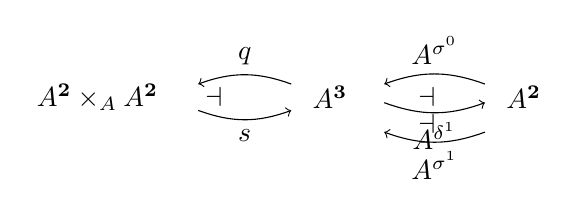
\begin{tikzpicture}[x=1.4em,y=1.4em]
  \node (L) at (0,0) {$A^{\qcTwo}\times_{A}A^{\qcTwo}$};
  \node (M) at (6.0,0) {$A^{\qcThree}$};
  \node (R) at (11.0,0) {$A^{\qcTwo}$};
  \draw[->] (5.0,0.34) to[bend right=20] node[above]{$q$} (2.6,0.34);
  \node at (3.0,0) {$\dashv$};
  \draw[->] (2.6,-0.34) to[bend right=20] node[below]{$s$} (5.0,-0.34);
  \draw[->] (10.0,0.34) to[bend right=20] node[above]{$A^{\sigma^{0}}$} (7.4,0.34);
  \node at (8.5,0) {$\dashv$};
  \draw[->] (7.4,-0.14) to[bend right=20] node[below]{$A^{\delta^{1}}$} (10.0,-0.14);
  \node at (8.5,-0.7) {$\dashv$};
  \draw[->] (10.0,-0.9) to[bend left=20] node[below]{$A^{\sigma^{1}}$} (7.4,-0.9);
\end{tikzpicture}
\end{center}
\end{proof}

注意，\eqref{eq:composition-functor}的诸伴随\trFunctor{}与到 $A\times A$ 的%
\trEndpointEvaluation{}函子可交换。事实上，各\trUnit{}与\trCounit{}同样可以纤维化到 $A\times A$ 之上
（见例 3.6.13）。%

\subsection*{练习}

\begin{exercise}\label{ex:cotensor-2-functor}
本练习的目标是把\cref{rem:contravariant-adjunction-preservation}所讨论的对偶伴随
保持结果中最微妙的一条明确写出来。
\begin{enumerate}[label=(\roman*)]
\item 设 $\mathcal{K}$ 是一个\trInfinityCosmos{}，$A$ 是其中的一个\trInfinityCategory{}。
  证明：单纯\trCotensor{}经限制后定义一个\trTwoFunctor
  $A^{(-)}\colon\mathrm{h}\QCat^{op}\to\mathrm{h}\mathcal{K}$。
\item 论证 (i) 的\trTwoFunctor{}沿\trNerve{}嵌入可进一步限制，从而定义一个%
  \trTwoFunctor{} $A^{(-)}\colon\Cat^{op}\to\mathrm{h}\mathcal{K}$。
\item 结论：对下方左侧所示的 1-\trCategory{}之间的任何\trAdjunction{}，都存在
  右侧所示的\trInfinityCategory{}之间的诱导\trAdjunction{}：
\begin{center}
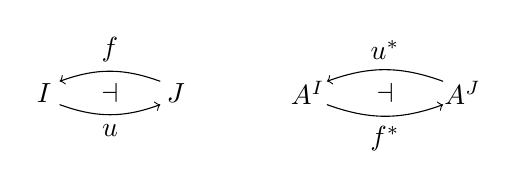
\begin{tikzpicture}[x=1.4em,y=1.4em]
  \node (I) at (0,0) {$I$};
  \node (J) at (3.4,0) {$J$};
  \draw[->] (3.0,0.3) to[bend right=20] node[above]{$f$} (0.4,0.3);
  \node at (1.7,0) {$\dashv$};
  \draw[->] (0.4,-0.3) to[bend right=20] node[below]{$u$} (3.0,-0.3);
  \node at (5.1,0) {$\rightsquigarrow$};
  \node (AI) at (6.8,0) {$A^{I}$};
  \node (AJ) at (10.8,0) {$A^{J}$};
  \draw[->] (10.3,0.3) to[bend right=20] node[above]{$u^{\ast}$} (7.3,0.3);
  \node at (8.8,0) {$\dashv$};
  \draw[->] (7.3,-0.3) to[bend right=20] node[below]{$f^{\ast}$} (10.3,-0.3);
\end{tikzpicture}
\end{center}
\end{enumerate}
\end{exercise}

\begin{exercise}\label{ex:uniqueness-converse}
证明\cref{prop:uniqueness-of-adjoints}(ii)。
\end{exercise}

\begin{exercise}\label{ex:dual-minimal-data}
把\cref{lem:minimal-adjunction-data}的证明对偶化，使之适用于
\cref{prop:adjoint-equivalences}的情形，从而证明：任何\trEquivalence{}都可提升为一个%
\trAdjointEquivalence{}，其中\trCounit{}是原先给定数据的一部分。
\end{exercise}

\begin{exercise}\label{ex:adjoint-equivalence-homotopy-category}
证明：\trInfinityCategory{}之间的\trAdjointEquivalence{}下降为相应\trHomotopyCategory{}之间的%
\trAdjointEquivalence{}。
\end{exercise}
